\documentclass[11pt]{article}
\usepackage[margin=0.85in]{geometry}
\usepackage{amsmath, amssymb}
\usepackage{xcolor}
\usepackage{tcolorbox}
\usepackage{enumitem}
\usepackage{multicol}
\usepackage{tikz}
\usepackage{fontenc}
\usepackage{inputenc}
\usepackage{fancyhdr}

\pagestyle{fancy}
\fancyhf{}
\fancyhead[L]{\textbf{Chapter 12 Practice}}
\fancyhead[R]{FangMath}
\fancyfoot[C]{\thepage}

% ── Colors ───────────────────────────────────────────────────────────────────
\definecolor{day1}{RGB}{26,35,126}
\definecolor{day2}{RGB}{0,105,62}
\definecolor{day3}{RGB}{130,0,0}
\definecolor{day4}{RGB}{100,50,0}
\definecolor{day5}{RGB}{60,20,100}
\definecolor{ltgray}{RGB}{245,245,245}
\definecolor{mygray}{RGB}{117,117,117}
\definecolor{anscolor}{RGB}{46,125,50}

\tcbuselibrary{skins}

\newcommand{\dayhdr}[3]{%
  \newpage
  \noindent\colorbox{#2}{\parbox{\linewidth}{%
    \vspace{6pt}\hspace{8pt}
    {\LARGE\textbf{\textcolor{white}{#1}}}
    \hfill
    {\normalsize\textcolor{white}{#3}}
    \vspace{6pt}
  }}
  \vspace{4pt}
}

\newcommand{\sechdr}[2]{%
  \vspace{8pt}
  \noindent\colorbox{#2}{\parbox{\linewidth}{%
    \vspace{3pt}\hspace{6pt}{\normalsize\textbf{\textcolor{white}{#1}}}\vspace{3pt}
  }}
  \vspace{4pt}
}

\newtcolorbox{ansbox}{
  colback=ltgray, colframe=anscolor, boxrule=0.8pt,
  arc=3pt, left=6pt, right=6pt, top=4pt, bottom=4pt,
  fontupper=\small\color{anscolor}
}

\newcommand{\ws}{\vspace{2.2cm}}   % work space
\newcommand{\wsl}{\vspace{3cm}}    % larger work space

\begin{document}

% ════════════════════════════════════════════════════════════════════════════
%  COVER
% ════════════════════════════════════════════════════════════════════════════
\begin{center}
  {\Huge\textbf{\textcolor{day1}{Chapter 12}}}\\[6pt]
  {\LARGE\textbf{5-Day Practice Set}}\\[4pt]
  {\large Radicals, Pythagorean Theorem \& Square Root Functions}\\[8pt]
  \rule{\linewidth}{2pt}
\end{center}

\medskip
\noindent\textbf{Name:}~\underline{\hspace{5cm}}
\quad\textbf{Date:}~\underline{\hspace{3cm}}
\quad\textbf{Period:}~\underline{\hspace{2cm}}

\bigskip
\begin{center}
\renewcommand{\arraystretch}{1.6}
\begin{tabular}{|c|c|c|c|}
\hline
\textbf{Day} & \textbf{Topics} & \textbf{Score} & \textbf{Date} \\
\hline
Day 1 & Foundation & \quad /10 & \\
\hline
Day 2 & Developing & \quad /10 & \\
\hline
Day 3 & Intermediate & \quad /10 & \\
\hline
Day 4 & Advanced & \quad /10 & \\
\hline
Day 5 & Challenge & \quad /10 & \\
\hline
\end{tabular}
\end{center}

\bigskip
\noindent\textbf{Topics covered each day:}
\begin{itemize}[itemsep=2pt]
  \item \textbf{A.} Finding the missing side of a right triangle (Pythagorean Theorem)
  \item \textbf{B.} State whether the given lengths can be sides of a right triangle
  \item \textbf{C.} Simplify radical expressions
  \item \textbf{D.} Solve radical equations
  \item \textbf{E.} Graph square root functions
\end{itemize}

% ════════════════════════════════════════════════════════════════════════════
%  DAY 1 — FOUNDATION
% ════════════════════════════════════════════════════════════════════════════
\dayhdr{Day 1 \quad Foundation}{day1}{10 problems · Easy}

\sechdr{Section A: Find the Missing Side Length}{day1}

\noindent\textit{Use $a^2 + b^2 = c^2$, where $c$ is the hypotenuse.}
\medskip

\begin{enumerate}[label=\textbf{\arabic*.}, itemsep=0pt]

  \item $a = 3,\ b = 4$. \; Find $c$.
  \ws

  \item $a = 5,\ c = 13$. \; Find $b$.
  \ws

\end{enumerate}

\sechdr{Section B: Is It a Right Triangle?}{day1}

\noindent\textit{Check whether $a^2 + b^2 = c^2$ holds (use the longest side as $c$).}
\medskip

\begin{enumerate}[label=\textbf{\arabic*.}, start=3, itemsep=0pt]

  \item $8,\ 15,\ 17$
  \ws

  \item $3,\ 5,\ 6$
  \ws

\end{enumerate}

\sechdr{Section C: Simplify Each Radical Expression}{day1}

\begin{enumerate}[label=\textbf{\arabic*.}, start=5, itemsep=0pt]

  \item $\sqrt{28}$
  \ws

  \item $\sqrt{75}$
  \ws

  \item $\sqrt{2} + \sqrt{8}$
  \ws

\end{enumerate}

\sechdr{Section D: Solve the Radical Equation}{day1}

\begin{enumerate}[label=\textbf{\arabic*.}, start=8, itemsep=0pt]

  \item $\sqrt{x} = 6$
  \ws

  \item $\sqrt{x} - 1 = 4$
  \ws

\end{enumerate}

\sechdr{Section E: Graph the Square Root Function}{day1}

\begin{enumerate}[label=\textbf{\arabic*.}, start=10, itemsep=0pt]

  \item Graph $y = \sqrt{x}$. \; Complete the table, then sketch.

  \medskip
  \begin{center}
  \renewcommand{\arraystretch}{2}
  \begin{tabular}{|c|c|c|c|c|}
  \hline
  $x$ & $0$ & $1$ & $4$ & $9$ \\
  \hline
  $y$ & & & & \\
  \hline
  \end{tabular}
  \end{center}

  \medskip
  \begin{center}
  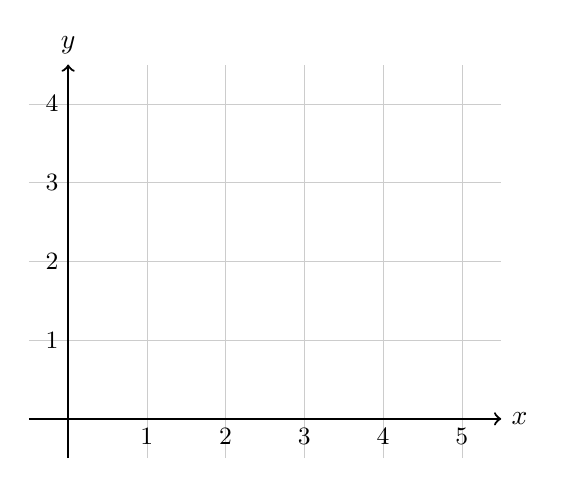
\begin{tikzpicture}
    \draw[very thin, gray!40] (-0.5,-0.5) grid (5.5,4.5);
    \draw[->, thick] (-0.5,0)--(5.5,0) node[right]{$x$};
    \draw[->, thick] (0,-0.5)--(0,4.5) node[above]{$y$};
    \foreach \x in {1,2,3,4,5} \node[below, font=\small] at (\x,0) {\x};
    \foreach \y in {1,2,3,4} \node[left,  font=\small] at (0,\y) {\y};
  \end{tikzpicture}
  \end{center}

  \noindent Domain: \underline{\hspace{4cm}} \quad Range: \underline{\hspace{4cm}}

\end{enumerate}

% ════════════════════════════════════════════════════════════════════════════
%  DAY 2 — DEVELOPING
% ════════════════════════════════════════════════════════════════════════════
\dayhdr{Day 2 \quad Developing}{day2}{10 problems · Easy--Medium}

\sechdr{Section A: Find the Missing Side Length}{day2}

\begin{enumerate}[label=\textbf{\arabic*.}, itemsep=0pt]

  \item $a = 9,\ b = 12$. \; Find $c$.
  \ws

  \item $b = 7,\ c = 25$. \; Find $a$.
  \ws

\end{enumerate}

\sechdr{Section B: Is It a Right Triangle?}{day2}

\begin{enumerate}[label=\textbf{\arabic*.}, start=3, itemsep=0pt]

  \item $1.5,\ 2.0,\ 2.5$
  \ws

  \item $5,\ 6,\ 8$
  \ws

\end{enumerate}

\sechdr{Section C: Simplify Each Radical Expression}{day2}

\begin{enumerate}[label=\textbf{\arabic*.}, start=5, itemsep=0pt]

  \item $\sqrt{300}$
  \ws

  \item $3\sqrt{5} + \sqrt{45}$
  \ws

  \item $4\sqrt{10} - \sqrt{40}$
  \ws

\end{enumerate}

\sechdr{Section D: Solve the Radical Equation}{day2}

\begin{enumerate}[label=\textbf{\arabic*.}, start=8, itemsep=0pt]

  \item $\sqrt{x + 3} = 5$
  \ws

  \item $2\sqrt{x} = 10$
  \ws

\end{enumerate}

\sechdr{Section E: Graph the Square Root Function}{day2}

\begin{enumerate}[label=\textbf{\arabic*.}, start=10, itemsep=0pt]

  \item Graph $y = \sqrt{x + 2}$. \; Complete the table, then sketch.

  \medskip
  \begin{center}
  \renewcommand{\arraystretch}{2}
  \begin{tabular}{|c|c|c|c|c|}
  \hline
  $x$ & $-2$ & $-1$ & $2$ & $7$ \\
  \hline
  $y$ & & & & \\
  \hline
  \end{tabular}
  \end{center}

  \medskip
  \begin{center}
  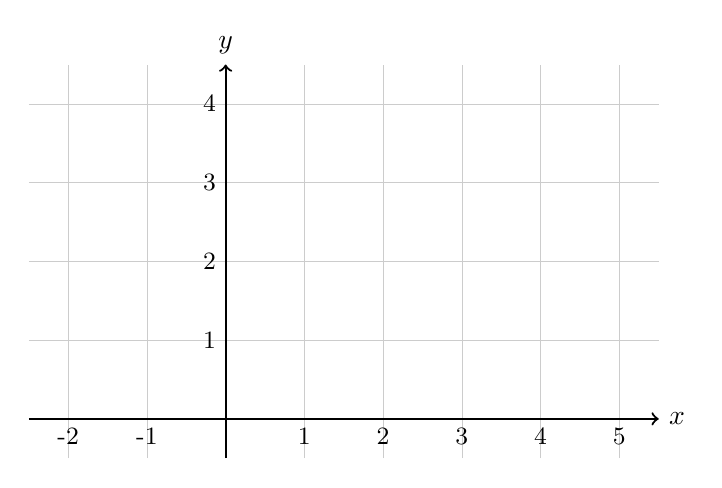
\begin{tikzpicture}
    \draw[very thin, gray!40] (-2.5,-0.5) grid (5.5,4.5);
    \draw[->, thick] (-2.5,0)--(5.5,0) node[right]{$x$};
    \draw[->, thick] (0,-0.5)--(0,4.5) node[above]{$y$};
    \foreach \x in {-2,-1,1,2,3,4,5} \node[below, font=\small] at (\x,0) {\x};
    \foreach \y in {1,2,3,4} \node[left, font=\small] at (0,\y) {\y};
  \end{tikzpicture}
  \end{center}

  \noindent Domain: \underline{\hspace{4cm}} \quad Range: \underline{\hspace{4cm}}

\end{enumerate}

% ════════════════════════════════════════════════════════════════════════════
%  DAY 3 — INTERMEDIATE
% ════════════════════════════════════════════════════════════════════════════
\dayhdr{Day 3 \quad Intermediate}{day3}{10 problems · Medium}

\sechdr{Section A: Find the Missing Side Length (Round to Nearest Tenth)}{day3}

\begin{enumerate}[label=\textbf{\arabic*.}, itemsep=0pt]

  \item $a = 7,\ b = 9$. \; Find $c$.
  \ws

  \item $a = 4.0,\ c = 4.1$. \; Find $b$.
  \ws

\end{enumerate}

\sechdr{Section B: Is It a Right Triangle?}{day3}

\begin{enumerate}[label=\textbf{\arabic*.}, start=3, itemsep=0pt]

  \item $7,\ 24,\ 25$
  \ws

  \item $8,\ 16,\ 17$
  \ws

\end{enumerate}

\sechdr{Section C: Simplify Each Radical Expression}{day3}

\begin{enumerate}[label=\textbf{\arabic*.}, start=5, itemsep=0pt]

  \item $\sqrt{3} + \sqrt{12}$
  \ws

  \item $\dfrac{-\sqrt{18}}{\sqrt{12}}$
  \ws

  \item $\dfrac{1}{\sqrt{3} + 4}$ \quad (rationalize the denominator)
  \ws

\end{enumerate}

\sechdr{Section D: Solve the Radical Equation. Check your solution.}{day3}

\begin{enumerate}[label=\textbf{\arabic*.}, start=8, itemsep=0pt]

  \item $\sqrt{2x} + 3 = 7$
  \ws

  \item $\dfrac{\sqrt{3m + 2}}{3} = 1$
  \wsl

\end{enumerate}

\sechdr{Section E: Graph the Square Root Function}{day3}

\begin{enumerate}[label=\textbf{\arabic*.}, start=10, itemsep=0pt]

  \item Graph $y = \sqrt{x - 3}$. \; Complete the table, then sketch.

  \medskip
  \begin{center}
  \renewcommand{\arraystretch}{2}
  \begin{tabular}{|c|c|c|c|c|}
  \hline
  $x$ & $3$ & $4$ & $7$ & $12$ \\
  \hline
  $y$ & & & & \\
  \hline
  \end{tabular}
  \end{center}

  \medskip
  \begin{center}
  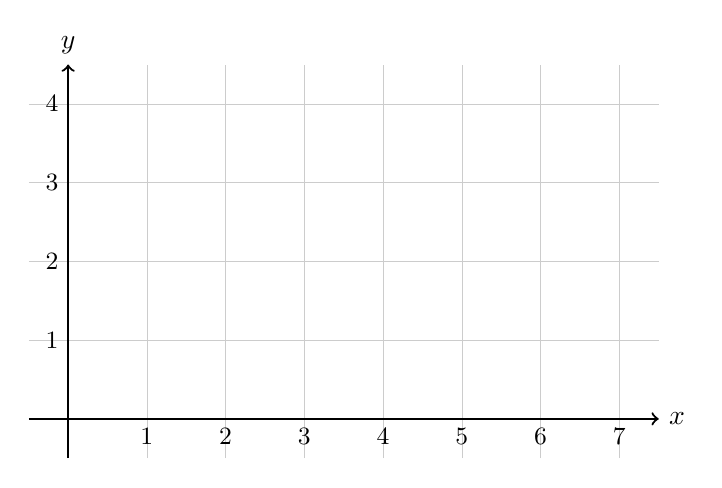
\begin{tikzpicture}
    \draw[very thin, gray!40] (-0.5,-0.5) grid (7.5,4.5);
    \draw[->, thick] (-0.5,0)--(7.5,0) node[right]{$x$};
    \draw[->, thick] (0,-0.5)--(0,4.5) node[above]{$y$};
    \foreach \x in {1,2,3,4,5,6,7} \node[below, font=\small] at (\x,0) {\x};
    \foreach \y in {1,2,3,4} \node[left, font=\small] at (0,\y) {\y};
  \end{tikzpicture}
  \end{center}

  \noindent Domain: \underline{\hspace{4cm}} \quad Range: \underline{\hspace{4cm}}

\end{enumerate}

% ════════════════════════════════════════════════════════════════════════════
%  DAY 4 — ADVANCED
% ════════════════════════════════════════════════════════════════════════════
\dayhdr{Day 4 \quad Advanced}{day4}{10 problems · Medium--Hard}

\sechdr{Section A: Find the Missing Side Length}{day4}

\begin{enumerate}[label=\textbf{\arabic*.}, itemsep=0pt]

  \item In a right triangle, one leg $= 20$ and the hypotenuse $= 21$. Find the other leg. Round to the nearest tenth.
  \ws

  \item \textbf{Word problem:} A 17-foot ladder leans against a wall. The base of the ladder is 8 feet from the wall. How high up the wall does the ladder reach?
  \wsl

\end{enumerate}

\sechdr{Section B: Is It a Right Triangle?}{day4}

\begin{enumerate}[label=\textbf{\arabic*.}, start=3, itemsep=0pt]

  \item $0.9,\ 1.2,\ 1.5$
  \ws

  \item $11,\ 13,\ 17$
  \ws

\end{enumerate}

\sechdr{Section C: Simplify Each Radical Expression}{day4}

\begin{enumerate}[label=\textbf{\arabic*.}, start=5, itemsep=0pt]

  \item $\dfrac{\sqrt{6}}{4 - \sqrt{6}}$ \quad (rationalize the denominator)
  \ws

  \item $\dfrac{\sqrt{2}}{\sqrt{2} + 3}$ \quad (rationalize the denominator)
  \ws

  \item $-3\sqrt{5x^3} \cdot \sqrt{10x^3}$
  \ws

\end{enumerate}

\sechdr{Section D: Solve the Radical Equation. Check for extraneous solutions.}{day4}

\begin{enumerate}[label=\textbf{\arabic*.}, start=8, itemsep=0pt]

  \item $\sqrt{2x + 4} = \sqrt{3x}$
  \wsl

  \item $\sqrt{2 - x} = x$
  \wsl

\end{enumerate}

\sechdr{Section E: Graph the Square Root Function}{day4}

\begin{enumerate}[label=\textbf{\arabic*.}, start=10, itemsep=0pt]

  \item Graph $y = \sqrt{x} + 5$. \; Complete the table, then sketch.

  \medskip
  \begin{center}
  \renewcommand{\arraystretch}{2}
  \begin{tabular}{|c|c|c|c|c|}
  \hline
  $x$ & $0$ & $1$ & $4$ & $9$ \\
  \hline
  $y$ & & & & \\
  \hline
  \end{tabular}
  \end{center}

  \medskip
  \begin{center}
  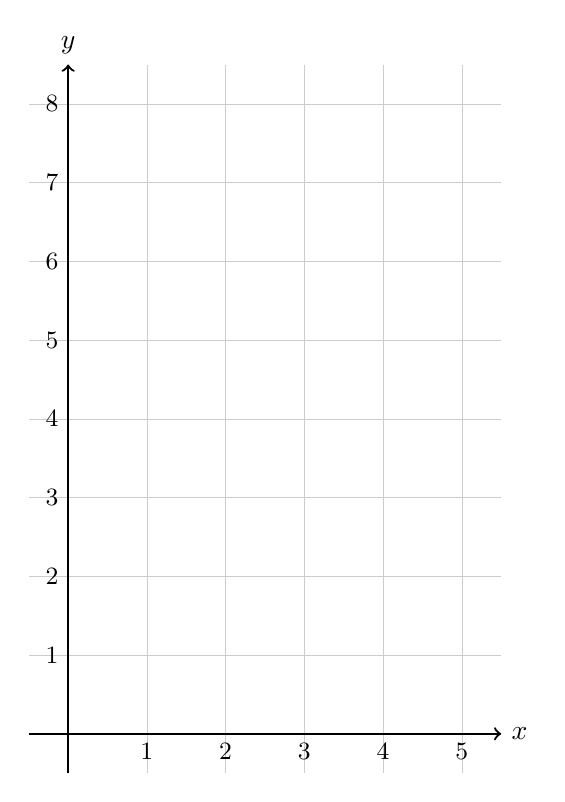
\begin{tikzpicture}
    \draw[very thin, gray!40] (-0.5,-0.5) grid (5.5,8.5);
    \draw[->, thick] (-0.5,0)--(5.5,0) node[right]{$x$};
    \draw[->, thick] (0,-0.5)--(0,8.5) node[above]{$y$};
    \foreach \x in {1,2,3,4,5} \node[below, font=\small] at (\x,0) {\x};
    \foreach \y in {1,...,8} \node[left, font=\small] at (0,\y) {\y};
  \end{tikzpicture}
  \end{center}

  \noindent Domain: \underline{\hspace{3.5cm}} \quad Range: \underline{\hspace{3.5cm}} \quad Starting point: \underline{\hspace{2cm}}

\end{enumerate}

% ════════════════════════════════════════════════════════════════════════════
%  DAY 5 — CHALLENGE
% ════════════════════════════════════════════════════════════════════════════
\dayhdr{Day 5 \quad Challenge}{day5}{10 problems · Hard}

\sechdr{Section A: Find the Missing Side Length}{day5}

\begin{enumerate}[label=\textbf{\arabic*.}, itemsep=0pt]

  \item \textbf{Word problem:} A baseball diamond is a square with 90-foot sides. How far is it from home plate to second base? (Hint: the diagonal of the square is the hypotenuse.) Round to the nearest tenth.
  \wsl

  \item \textbf{Word problem:} Two hikers leave from the same point. One walks 12 miles north and the other walks 16 miles east. How far apart are they?
  \wsl

\end{enumerate}

\sechdr{Section B: Is It a Right Triangle? (These involve non-integer sides.)}{day5}

\begin{enumerate}[label=\textbf{\arabic*.}, start=3, itemsep=0pt]

  \item $\sqrt{2},\ \sqrt{3},\ \sqrt{5}$
  \ws

  \item $\sqrt{3},\ 2,\ \sqrt{6}$ \quad (Is $(\sqrt{3})^2 + 2^2 = (\sqrt{6})^2$?)
  \ws

\end{enumerate}

\sechdr{Section C: Simplify Each Radical Expression}{day5}

\begin{enumerate}[label=\textbf{\arabic*.}, start=5, itemsep=0pt]

  \item $\dfrac{\sqrt{5} - \sqrt{3}}{\sqrt{5} + \sqrt{3}}$ \quad (rationalize the denominator)
  \ws

  \item $\dfrac{3}{2\sqrt{3} - \sqrt{2}}$ \quad (rationalize the denominator)
  \ws

  \item $\sqrt{2x + 4} \cdot \sqrt{8x + 16}$ \quad (simplify completely)
  \ws

\end{enumerate}

\sechdr{Section D: Solve the Radical Equation. Check for extraneous solutions.}{day5}

\begin{enumerate}[label=\textbf{\arabic*.}, start=8, itemsep=0pt]

  \item $\sqrt{-5a + 6} = -a$
  \wsl

  \item $\sqrt{x + 5} + \sqrt{x} = 5$
  \wsl

\end{enumerate}

\sechdr{Section E: Graph the Square Root Function}{day5}

\begin{enumerate}[label=\textbf{\arabic*.}, start=10, itemsep=0pt]

  \item Graph $y = \sqrt{x + 4} - 2$. \; Complete the table, then sketch.

  \medskip
  \begin{center}
  \renewcommand{\arraystretch}{2}
  \begin{tabular}{|c|c|c|c|c|c|}
  \hline
  $x$ & $-4$ & $-3$ & $0$ & $5$ & $12$ \\
  \hline
  $y$ & & & & & \\
  \hline
  \end{tabular}
  \end{center}

  \medskip
  \begin{center}
  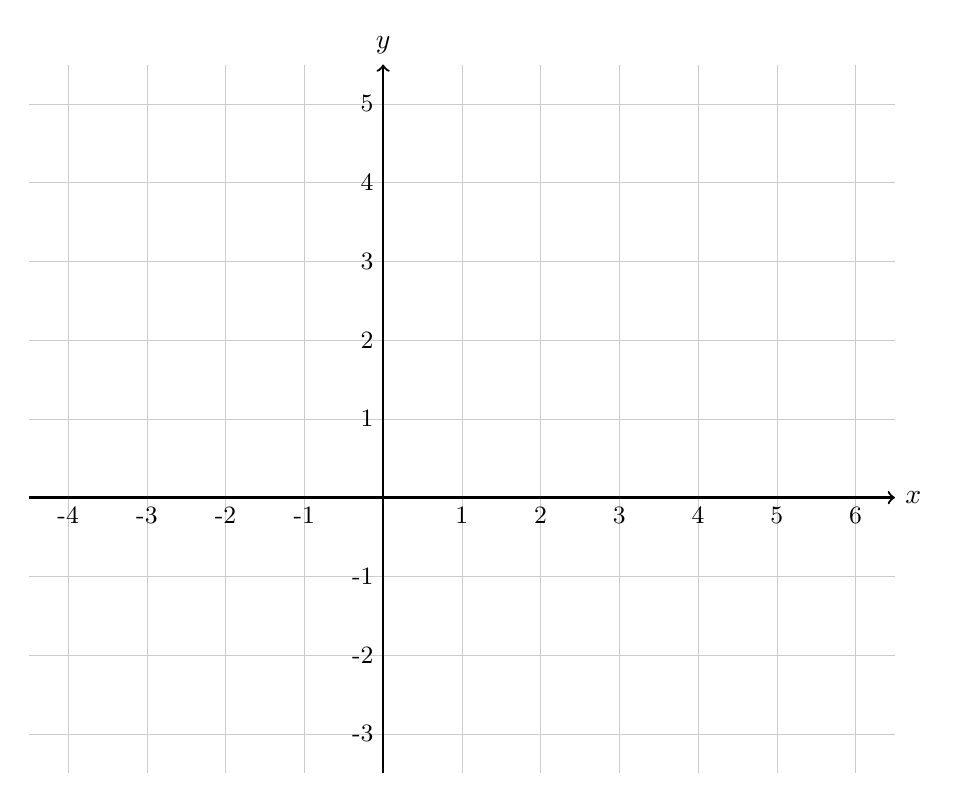
\begin{tikzpicture}
    \draw[very thin, gray!40] (-4.5,-3.5) grid (6.5,5.5);
    \draw[->, thick] (-4.5,0)--(6.5,0) node[right]{$x$};
    \draw[->, thick] (0,-3.5)--(0,5.5) node[above]{$y$};
    \foreach \x in {-4,-3,-2,-1,1,2,3,4,5,6} \node[below, font=\small] at (\x,0) {\x};
    \foreach \y in {-3,-2,-1,1,2,3,4,5} \node[left, font=\small] at (0,\y) {\y};
  \end{tikzpicture}
  \end{center}

  \noindent Domain: \underline{\hspace{3cm}} \; Range: \underline{\hspace{3cm}} \; Starting point: \underline{\hspace{2cm}}

\end{enumerate}

% ════════════════════════════════════════════════════════════════════════════
%  ANSWER KEY
% ════════════════════════════════════════════════════════════════════════════
\newpage
\begin{center}
{\Large\textbf{\textcolor{day1}{Answer Key}}}\\[4pt]
\rule{\linewidth}{1.5pt}
\end{center}

\medskip
\begin{ansbox}
\textbf{Day 1:} \quad
1.~$c=5$ \quad
2.~$b=12$ \quad
3.~Yes \quad
4.~No \quad
5.~$2\sqrt{7}$ \quad
6.~$5\sqrt{3}$ \quad
7.~$3\sqrt{2}$ \quad
8.~$x=36$ \quad
9.~$x=25$ \quad
10.~Domain $x\ge0$, Range $y\ge0$
\end{ansbox}

\medskip
\begin{ansbox}
\textbf{Day 2:} \quad
1.~$c=15$ \quad
2.~$a=24$ \quad
3.~Yes \quad
4.~No \quad
5.~$10\sqrt{3}$ \quad
6.~$6\sqrt{5}$ \quad
7.~$2\sqrt{10}$ \quad
8.~$x=22$ \quad
9.~$x=25$ \quad
10.~Domain $x\ge-2$, Range $y\ge0$
\end{ansbox}

\medskip
\begin{ansbox}
\textbf{Day 3:} \quad
1.~$c\approx11.4$ \quad
2.~$b=0.9$ \quad
3.~Yes \quad
4.~No \quad
5.~$3\sqrt{3}$ \quad
6.~$-\dfrac{\sqrt{6}}{2}$ \quad
7.~$\dfrac{4-\sqrt{3}}{13}$ \quad
8.~$x=8$ \quad
9.~$m=\dfrac{7}{3}$ \quad
10.~Domain $x\ge3$, Range $y\ge0$
\end{ansbox}

\medskip
\begin{ansbox}
\textbf{Day 4:} \quad
1.~$\approx6.4$ \quad
2.~$15$ ft \quad
3.~Yes \quad
4.~No \quad
5.~$\dfrac{2\sqrt{6}+3}{5}$ \quad
6.~$\dfrac{3\sqrt{2}-2}{7}$ \quad
7.~$-15x^3\sqrt{2}$ \quad
8.~$x=4$ \quad
9.~$x=1$ (check: $x=-2$ is extraneous) \quad
10.~Domain $x\ge0$, Range $y\ge5$, Start $(0,5)$
\end{ansbox}

\medskip
\begin{ansbox}
\textbf{Day 5:} \quad
1.~$90\sqrt{2}\approx127.3$ ft \quad
2.~$20$ miles \quad
3.~Yes ($2+3=5$) \quad
4.~No ($3+4=7\ne6$) \quad
5.~$4-\sqrt{15}$ \quad
6.~$\dfrac{6\sqrt{3}+3\sqrt{2}}{10}$ \quad
7.~$4|x+2|$ \quad
8.~$a=-6$ ($a=1$ extraneous) \quad
9.~$x=4$ \quad
10.~Domain $x\ge-4$, Range $y\ge-2$, Start $(-4,-2)$
\end{ansbox}

\end{document}
